\subsection{The CML Metamodel (Abstract Syntax)}\label{subsec:metamodel}

In the article \emph{UML and OCL in Conceptual Modeling}, 
Gogolla \cite{gogolla} shows, by mapping the UML \cite{uml} metamodel to the ER \cite{er} metamodel,
how UML models (augmented by OCL \cite{ocl} constraints) can be used to specify conceptual models.
Also, Wazlawick \cite{wazlawick} systematically prescribes in his book a method for conceptual modeling using UML and OCL. 

Since one key CML goal is enabling the specification of conceptual models
(such as those specified by ER models and UML/OCL models),
in order to present the key elements of the CML metamodel,
a similar approach to Gogolla's is used to map the CML metamodel to the ER metamodel,
and to the UML/OCL metamodel.

\pagebreak[4]

The EMOF \cite{mof} model presented by figure \ref{fig:metamodel} is a simplified version of the CML metamodel:

\begin{figure}
\centering
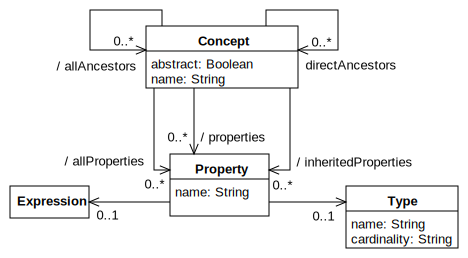
\includegraphics[width=0.8\textwidth]{language/diagram-metamodel}
\caption{This class diagram renders the EMOF \cite{mof} model defining the CML metamodel.}
\label{fig:metamodel}
\end{figure}

In CML metamodel shown in figure \ref{fig:metamodel},
a \emph{Concept} is composed of zero-or-more \emph{Property} instances.
Each \emph{Property} may have a \emph{Type} and an \emph{Expression}.
If two \emph{Property} instances represent the same bidirectional association,
there must be an \emph{Association} instance that binds them.
Unidirectional associations are only represented by the \emph{Property} instance (representing the association role)
that enables the navigation from the source \emph{Concept} instance to the target one (which is represented by the property's \emph{Type}.)

Next, there is a description for each metamodel element. \emph{Expression} will be covered in subsection \ref{subsec:expr}.

\subsubsection{Concept}
\subsubsection{Property}
\subsubsection{Association}
\subsubsection{Type}
